
关于CMake的在线参考将建议使用ExternalProject和FetchContent模块来处理更复杂项目中的依赖性管理。这是一个很好的建议,但通常是在没有给出相应的使用背景,这就出现了很多问题。这些模块是干什么用的?什么时候选择这一个,而不是另一个?它们究竟是如何工作的,之间又是如何相互作用的?有些答案比其他的更难找到,并且CMake的文档并没有对这个主题提供一个清晰的介绍,但这里会给出。

\subsubsubsection{7.6.1\hspace{0.2cm}ExternalProject}

CMake 3.0.0引入了名为ExternalProject的模块,目的是添加对在线存储库中可用的外部项目的支持。随着时间的推移,该模块逐渐扩展以满足不同的需求,产生了相当复杂的命令——ExternalProject\_Add()。因为它提供了一系列令人印象深刻的功能,并且可以接受超过85种不同的选择:

\begin{itemize}
\item 
管理外部项目的目录结构

\item 
从URL下载源代码(若需要,还可以从压缩包中提取)

\item 
支持Git、Subversion、Mercurial和CVS库

\item 
若需要,可以获取更新

\item 
使用CMake、Make或用户指定的工具配置和构建项目

\item 
执行安装和运行测试

\item 
日志文件

\item 
终端请求用户输入

\item 
依赖于其他目标

\item 
向构建中添加自定义命令/步骤
\end{itemize}

ExternalProject模块在构建阶段填充依赖项。对于ExternalProject\_Add()添加的每个外部项目,CMake将执行以下步骤:


\begin{enumerate}
\item 
mkdir – 为外部项目创建子目录

\item 
download – 从存储库或URL获取项目文件

\item 
update – 重新运行时支持增量更新的下载方式

\item 
patch – 可选地执行一个补丁命令,根据项目的需要更改下载的文件

\item 
configure – 执行CMake项目的配置阶段,或者手动指定非CMake依赖项的命令

\item 
build – 执行CMake项目的构建阶段,而对于其他依赖项,执行make命令

\item 
install – 安装CMake项目,对于其他依赖,执行make install命令

\item 
test – 若选择性的定义了TEST\_…,则执行依赖项的测试
\end{enumerate}

除测试步骤外,其他步骤完全遵循上述顺序,测试步骤可以通过TEST\_BEFORE\_INSTALL <bool>或TEST\_AFTER\_INSTALL <bool>选项在安装步骤之前或之后启用。

\hspace*{\fill} \\ %插入空行
\noindent
\textbf{下载步骤选项}

最有趣的是控制下载步骤的选项,或者CMake如何获取依赖项。首先,可以选择不使用CMake内置方法,而使用一个自定义指令(这里支持生成器表达式):

\begin{lstlisting}[style=styleCMake]
DOWNLOAD_COMMAND <cmd>...
\end{lstlisting} 

这就是告诉CMake忽略此步骤的所有其他选项,只执行一个特定于系统的命令。也接受空字符串,用于禁用此步骤。

\hspace*{\fill} \\ %插入空行
\noindent
\textbf{使用URL下载依赖项}

可以提供一个按顺序扫描的URL列表,直到下载成功。CMake会识别下载的文件是否是压缩包,并在默认情况下将其解包:

\begin{lstlisting}[style=styleCMake]
URL <url1> [<url2>...]
\end{lstlisting} 

一些选项允许进一步定制化这个方法的行为:

\begin{itemize}
\item 
URL\_HASH <algo>=<hashValue> – 检查<algo>生成的下载文件的校验和是否与提供的匹配,这里建议检查下载文件的完整性。MD5、SHA1、SHA224、SHA256、SHA384、SHA512、SHA3\_224、SHA3\_256、SHA3\_384和SHA3\_512支持的算法由string()指令定义。对于MD5,可以使用简写选项URL\_MD5 <MD5>。

\item 
DOWNLOAD\_NO\_EXTRACT <bool> -下载后显式禁用提取。可以在后续步骤中通过访问<DOWNLOADED\_FILE>来使用下载文件的文件名。

\item 
DOWNLOAD\_NO\_PROGRESS <bool> – 不显示下载进度。

\item 
TIMEOUT <seconds> 和 INACTIVITY\_TIMEOUT <seconds> – 超时后终止在固定时间或不活动期间后的下载。

\item 
HTTP\_USERNAME <username> 和 HTTP\_PASSWORD <password> – 选项为HTTP身份验证提供值,要避免在项目中硬编码凭证。

\item 
HTTP\_HEADER <header1> [<header2>…] – 在HTTP请求中发送附加的报头,来访问AWS中的内容或传递一些自定义令牌。

\item 
TLS\_VERIFY <bool> – 验证SSL证书。若没有设置,CMake将从CMAKE\_TLS\_VERIFY变量中读取该设置,该变量默认设置为false。跳过TLS验证是一种不安全的做法,应该避免使用,特别是在生产环境中。

\item 
TLS\_CAINFO <file> – 若公司正在颁发自签名SSL证书,这将非常有用。该选项提供到授权文件的路径;若没有指定,CMake将从CMAKE\_TLS\_CAINFO中读取该设置。
\end{itemize}

\hspace*{\fill} \\ %插入空行
\noindent
\textbf{使用Git下载依赖项}

要从Git下载依赖项,需要确定主机安装了Git 1.6.5或更高版本。从Git中克隆需要以下选项:

\begin{lstlisting}[style=styleCMake]
GIT_REPOSITORY <url>
GIT_TAG <tag>
\end{lstlisting} 

<url>和<tag>都应该采用git命令能够理解的格式。此外,建议使用特定的git提交哈希,以确保生成的二进制文件可以跟踪到特定的提交,并且没有不必要的git获取执行。若坚持使用分支,请使用诸如origin/main这样的远程名称。这保证了本地克隆的正确同步。

其他选项如下:

\begin{itemize}
\item 
GIT\_REMOTE\_NAME <name> – 远程名称,默认为origin。

\item 
GIT\_SUBMODULES <module>... – 指定应该更新哪些子模块。从3.16开始,这个值默认为空(以前,所有子模块都更新了)。

\item 
GIT\_SUBMODULES\_RECURSE 1 – 启用子模块的递归更新。

\item 
GIT\_SHALLOW 1 – 执行浅克隆(不下载历史提交)。出于性能考虑,建议使用此选项。

\item 
TLS\_VERIFY <bool> – 从URL下载依赖项一节解释了这个选项。Git也可以使用,为了安全性应该启用。
\end{itemize}

\hspace*{\fill} \\ %插入空行
\noindent
\textbf{使用Subversion下载依赖项}

使用Subversion下载,应该指定以下选项:

\begin{lstlisting}[style=styleCMake]
SVN_REPOSITORY <url>
SVN_REVISION -r<rev>
\end{lstlisting} 

此外,可能需要提供以下信息:

\begin{itemize}
\item 
SVN\_USERNAME <user> 和 SVN\_PASSWORD <password> – 用于签出和更新的凭据,不过需要避免在项目中硬编码它们。
	
\item 
SVN\_TRUST\_CERT <bool> – 跳过Subversion服务器站点证书的验证。只有在到服务器的网络路径及其完整性是可信任的情况下才使用此选项。默认是禁用的。
\end{itemize}

\hspace*{\fill} \\ %插入空行
\noindent
\textbf{使用Mercurial下载依赖项}

这种模式非常简单,需要提供两个选项:

\begin{lstlisting}[style=styleCMake]
HG_REPOSITORY <url>
HG_TAG <tag>
\end{lstlisting} 

\hspace*{\fill} \\ %插入空行
\noindent
\textbf{使用CVS下载依赖项}

要检出CVS中的模块,需要提供以下三个选项:

\begin{lstlisting}[style=styleCMake]
CVS_REPOSITORY <cvsroot>
CVS_MODULE <module>
CVS_TAG <tag>
\end{lstlisting} 

\hspace*{\fill} \\ %插入空行
\noindent
\textbf{更新步骤选项}

若下载方法支持更新,更新步骤将重新下载外部项目的文件。可以用两种方式覆盖这种行为:

\begin{itemize}
\item 
用UPDATE\_COMMAND <cmd>提供在更新期间执行的自定义命令。

\item 
禁用更新步骤(以允许使用断开连接的网络构建)- UPDATE\_DISCONNECTED <bool>。请注意,下载步骤(在第一次构建期间)仍然会发生。
\end{itemize}

\hspace*{\fill} \\ %插入空行
\noindent
\textbf{补丁步骤选项}

这是一个可选步骤,将在获取源之后执行,需要指定想要执行的命令:

\begin{lstlisting}[style=styleCMake]
PATCH_COMMAND <cmd>...
\end{lstlisting} 

CMake文档警告说,有些补丁可能比其他补丁更“黏”。例如,在Git中,更改的文件在更新期间不会恢复到原始状态,需要小心避免两次错误地对文件打补丁。理想情况下,patch命令应该非常健壮。

\begin{tcolorbox}[colback=blue!5!white,colframe=blue!75!black,title=重要的Note]
前面提到的选项列表只包含最有用的条目。请务必参考官方文档了解更多细节和其他步骤的选项描述: \url{https://cmake.org/cmake/ help/latest/module/ExternalProject.html}.
\end{tcolorbox}

\hspace*{\fill} \\ %插入空行
\noindent
\textbf{使用ExternalProject}

依赖项在构建阶段创建,这样有两个效果——项目的命名空间完全独立,外部项目定义的目标在主项目中不可见。因为不能像使用find\_package()指令一样使用target\_link\_libraries(),所以后者尤其令人痛苦。没办法,因为两个构型阶段是分离的。在下载和配置依赖项之前,主项目必须完成配置阶段并启动构建阶段。这是一个问题,但我们会学习如何处理这个问题。现在,让我们看看ExternalProject\_Add()如何与前面的yaml-cpp库一起工作:

\begin{lstlisting}[style=styleCMake]
# chapter07/08-external-project-git/CMakeLists.txt

cmake_minimum_required(VERSION 3.20.0)
project(ExternalProjectGit CXX)

add_executable(welcome main.cpp)
configure_file(config.yaml config.yaml COPYONLY)

include(ExternalProject)
ExternalProject_Add(external-yaml-cpp
	GIT_REPOSITORY https://github.com/jbeder/yaml-cpp.git
	GIT_TAG yaml-cpp-0.6.3
)
target_link_libraries(welcome PRIVATE yaml-cpp)
\end{lstlisting} 

以下是构建此项目所采取的步骤:

\begin{itemize}
\item 
包含了ExternalProject模块来访问它的功能。

\item 
使用FindExternalProject\_Add(),该指令负责构建阶段下载必要的文件,并在系统中配置、构建和安装依赖项。
\end{itemize}

这里需要谨慎,并理解这个示例只能工作,因为yaml-cpp库在其CMakeLists.txt中定义了一个安装阶段。此阶段将库文件复制到系统中的标准位置。target\_link\_libraries()的yaml-cpp参数解释为链接器——-lyaml-cpp。此行为与前面的示例不同,前面的示例中,显式地定义了yaml-cpp目标。若库不提供安装阶段(或者二进制版本的名称不匹配),链接器就会出错。

现在,应该更深入地研究每个阶段的配置,并解释如何使用不同的下载方法。我们会在FetchContent部分讨论这个问题,回到ExternalProject获取依赖项的延迟问题,不能在编译阶段使用外部项目的目标,因为在获取这些项目时,编译阶段已经结束了。CMake将显式地保护用FindExternalProject\_Add()创建的目标,用一个特殊的UTILITY类型标记它。当错误地尝试在主项目中使用这样的目标时(可能链接),CMake将抛出一个错误:

\begin{tcblisting}{commandshell={}}
Target "external-yaml-cpp-build" of type UTILITY may not be
linked into another target.
\end{tcblisting}

为了避开这个限制,可以在技术上创建另一个目标,一个IMPORTED库,并使用它(就像使用FindPQXX.cmake那样),但这是一项非常艰巨的工作。更糟糕的是CMake实际上理解由外部CMake项目创建的目标(因为构建了它们)。主项目中重复这些声明并不是一个非常DRY的实践。

另一种可能的解决方案是将整个依赖项获取和构建提取到一个单独的子项目中,并在配置阶段构建该子项目,需要用execute\_process()启动另一个CMake实例。通过一些技巧和add\_subdirectory(),将这个子项目的列表文件和二进制文件消耗到主项目中。这种方法(有时称为超级构建)是过时的和不必要的。这里就不详细讲了,因为这对初学者来说没什么用。若有兴趣,可以读读Craig Scott这篇写的很棒的文章:\url{https://crascit.com/2015/07/25/cmake-gtest/}。

总而言之,当项目之间存在名称空间冲突时,ExternalProject可以让我们摆脱束缚,但FetchContent都要优雅得多。

\subsubsubsection{7.6.2\hspace{0.2cm}FetchContent}

现在,建议使用FetchContent模块来导入外部项目。这个模块从3.11版本就已经在CMake中可用了,但建议至少使用3.14才能有效地使用。

本质上,它是ExternalProject的高级包装器,提供类似的功能和更多功能。关键的区别在于执行阶段——与ExternalProject不同,FetchContent在配置阶段填充依赖项,将外部项目声明的所有目标带入主项目的范围。

FetchContent模块的使用需要三个步骤:

\begin{enumerate}
\item 
用include(FetchModule)将该模块包含到项目中。

\item 
使用FetchContent\_Declare()指令配置依赖项。

\item 
使用FetchContent\_MakeAvailable()指令填充依赖项——下载、构建、安装,并将其列表文件添加到主项目并进行解析。
\end{enumerate}

为什么Declare和MakeAvailable命令是分开的。这样做是为了在分层项目中启用配置重写。这里有一个场景——父项目依赖于A和B外部库。A库也依赖于B,但是A库的作者仍然使用旧版本,与父项目不同(图7.1):

\begin{center}
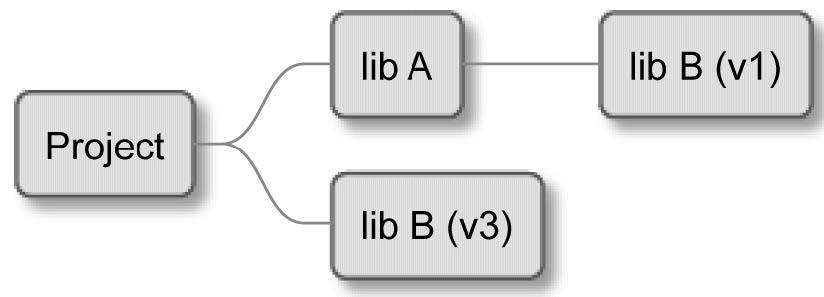
\includegraphics[width=0.5\textwidth]{content/2/chapter7/images/1.jpg}\\
图7.1 分层项目
\end{center}

而且对B库的依赖是可选的,取决于配置(假设特定于操作系统)。MakeAvailable不能同时配置和填充依赖项,因为要覆盖A库中的版本,父项目将填充依赖项,而不管它在A库中的最终需要。

由于有单独的配置步骤,能够在父项目中指定一个版本,并在所有子项目和依赖项中使用:

\begin{lstlisting}[style=styleCMake]
FetchContent_Declare(
	googletest
	GIT_REPOSITORY https://github.com/google/googletest.git
	# release-1.11.0
	GIT_TAG e2239ee6043f73722e7aa812a459f54a28552929
)
\end{lstlisting} 

使用googletest作为第一个参数对FetchContent\_Declare()的后续调用都将忽略,以允许层次结构中最高的项目决定如何处理该依赖项。

FetchContent\_Declare()的签名与ExternalProject\_Add()完全相同:

\begin{lstlisting}[style=styleCMake]
FetchContent_Declare(<depName> <contentOptions>...)
\end{lstlisting} 

这不是巧合——这些参数将存储起来,直到使用FetchContent\_MakeAvailable()。然后,变量将转发至ExternalProject\_Add()。然而,并不是所有的选项都允许转发。可以指定下载、更新或补丁步骤的任何选项,但不能指定配置、构建、安装或测试步骤。

当配置就绪时,可以这样填充依赖项:

\begin{lstlisting}[style=styleCMake]
FetchContent_MakeAvailable(<depName>)
\end{lstlisting} 

这将下载文件并将目标读取到项目中,但在调用期间发生了什么呢?在CMake 3.14中添加了FetchContent\_MakeAvailable()来将最常用的场景封装在指令中。图7.2中,可以看到整个过程的细节:

\begin{enumerate}
\item 
调用FetchContent\_GetProperties()将FetchContent\_Declare()设置的配置从全局变量读取到本地变量。

\item 
检查(不区分大小写)带有此名称的依赖项是否已经填充,以避免下载两次。

\item 
使用FetchContent\_Populate(),将通过转发设置的选项(但跳过禁用的选项)和下载依赖项来配置包装的ExternalProject模块。还会设置一些变量,以防止在后续调用中重新下载,并将必要的路径转发到下一个指令。

\item 
最后,使用源码树和构建树作为参数调用add\_subdirectory(),以告诉父项目列表文件在哪里,以及将构建构件放在哪里。
\end{enumerate}

通过调用add\_subdirectory(),有效地执行所获取项目的配置阶段,并检索在当前作用域中定义的目标。多方便啊!

\begin{center}
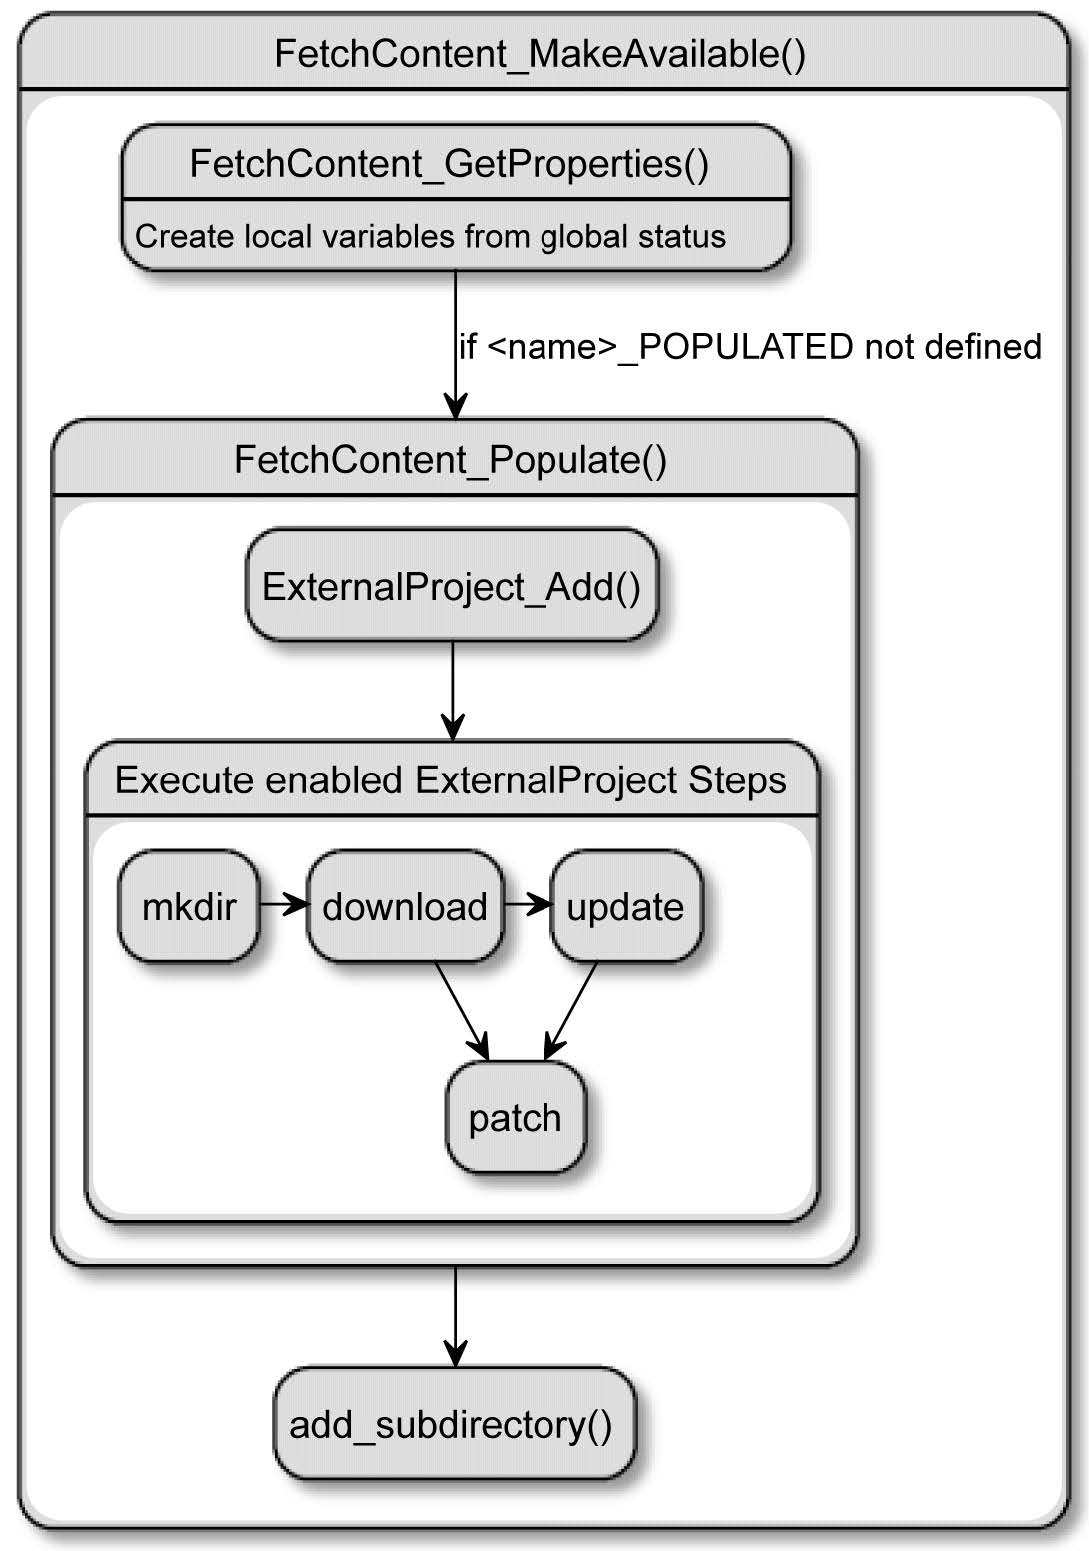
\includegraphics[width=0.6\textwidth]{content/2/chapter7/images/2.jpg}\\
图7.2  FetchContent\_MakeAvailable()如何包装对ExternalProject的调用
\end{center}

显然,可能会遇到这样的情况:两个不相关的项目声明一个同名目标。这是一个只能通过退回到ExternalProject或其他方法来解决的问题,但这种情况并不经常发生。

为了使这个解释完整,必须辅以一个实际的例子。来看看当切换到FetchContent时,前一节中的列表文件是如何变化的:

\begin{lstlisting}[style=styleCMake]
# chapter07/09-fetch-content/CMakeLists.txt

cmake_minimum_required(VERSION 3.20.0)
project(ExternalProjectGit CXX)

add_executable(welcome main.cpp)
configure_file(config.yaml config.yaml COPYONLY)

include(FetchContent)
FetchContent_Declare(external-yaml-cpp
	GIT_REPOSITORY https://github.com/jbeder/yaml-cpp.git
	GIT_TAG yaml-cpp-0.6.3
)
FetchContent_MakeAvailable(external-yaml-cpp)
target_link_libraries(welcome PRIVATE yaml-cpp)
\end{lstlisting} 

ExternalProject\_Add直接替换为FetchContent\_Declare,并且添加了另一个指令——FetchContent\_MakeAvailable。代码中的变化很小,但实际差异却是巨大的!可以显式访问由yaml-cpp库创建的目标。为了证明这一点,可以使用CMakePrintHelpers辅助模块,并在前面的文件中添加以下行:

\begin{lstlisting}[style=styleCMake]
include(CMakePrintHelpers)
cmake_print_properties(TARGETS yaml-cpp
	PROPERTIES TYPE SOURCE_DIR)
\end{lstlisting} 

现在,配置阶段将打印以下输出:

\begin{lstlisting}[style=styleCMake]
Properties for TARGET yaml-cpp:
	yaml-cpp.TYPE = "STATIC_LIBRARY"
	yaml-cpp.SOURCE_DIR = "/tmp/b/_deps/external-yaml-cpp-src"
\end{lstlisting} 

目标的存在,是一个静态库,源目录驻留在构建树中。使用相同的辅助函数来调试ExternalProject示例中的目标只会返回:

\begin{tcblisting}{commandshell={}}
No such TARGET "yaml-cpp" !
\end{tcblisting}

配置阶段无法识别目标。这就是为什么FetchContent要好得多,应该尽可能地使用它。




